\documentclass[dvips, lscape]{foils}
%\documentclass[dvips, french]{slides}
\textwidth 18.5cm
\textheight 25cm 
\topmargin -1cm 
\oddsidemargin  -1cm 
\evensidemargin  -1cm

% Maths
\usepackage{amsfonts, amsmath, amssymb}

\newcommand{\coefbin}[2]{\left( 
    \begin{array}{c} #1 \\ #2 \end{array} 
  \right)}
\newcommand{\Bcal}{\mathcal{B}}
\newcommand{\Ccal}{\mathcal{C}}
\newcommand{\Dcal}{\mathcal{D}}
\newcommand{\Ecal}{\mathcal{E}}
\newcommand{\Gcal}{\mathcal{G}}
\newcommand{\Mcal}{\mathcal{M}}
\newcommand{\Ncal}{\mathcal{N}}
\newcommand{\Pcal}{\mathcal{P}}
\newcommand{\Lcal}{\mathcal{L}}
\newcommand{\Tcal}{\mathcal{T}}
\newcommand{\Ucal}{\mathcal{U}}
\newcommand{\alphabf}{\mbox{\mathversion{bold}{$\alpha$}}}
\newcommand{\betabf}{\mbox{\mathversion{bold}{$\beta$}}}
\newcommand{\gammabf}{\mbox{\mathversion{bold}{$\gamma$}}}
\newcommand{\mubf}{\mbox{\mathversion{bold}{$\mu$}}}
\newcommand{\Pibf}{\mbox{\mathversion{bold}{$\Pi$}}}
\newcommand{\psibf}{\mbox{\mathversion{bold}{$\psi$}}}
\newcommand{\Sigmabf}{\mbox{\mathversion{bold}{$\Sigma$}}}
\newcommand{\taubf}{\mbox{\mathversion{bold}{$\tau$}}}
\newcommand{\Hbf}{{\bf H}}
\newcommand{\Ibf}{{\bf I}}
\newcommand{\Sbf}{{\bf S}}
\newcommand{\mbf}{{\bf m}}
\newcommand{\ubf}{{\bf u}}
\newcommand{\vbf}{{\bf v}}
\newcommand{\xbf}{{\bf x}}
\newcommand{\Xbf}{{\bf X}}
\newcommand{\Esp}{{\mathbb E}}
\newcommand{\Var}{{\mathbb V}}
\newcommand{\Cov}{{\mathbb C}\mbox{ov}}
\newcommand{\Ibb}{{\mathbb I}}
\newcommand{\Rbb}{\mathbb{R}}

% sommes
\newcommand{\sumk}{\sum_k}
\newcommand{\sumt}{\sum_{t \in I_k}}
\newcommand{\sumth}{\sum_{t=t_{k-1}^{(h)}+1}^{t_k^{(h)}}}
\newcommand{\sump}{\sum_{p=1}^{P}}
\newcommand{\suml}{\sum_{\ell=1}^{P}}
\newcommand{\sumtau}{\sum_k \hat{\tau}_{kp}}

% Couleur et graphiques
\usepackage{color}
\usepackage{graphics}
\usepackage{epsfig} 
\usepackage{pstcol}

% Texte
\usepackage{lscape}
\usepackage{../../../../Latex/fancyheadings, rotating, enumerate}
%\usepackage[french]{babel}
\usepackage[latin1]{inputenc}
\definecolor{darkgreen}{cmyk}{0.5, 0, 0.5, 0.5}
\definecolor{orange}{cmyk}{0, 0.6, 0.8, 0}
\definecolor{jaune}{cmyk}{0, 0.5, 0.5, 0}
\newcommand{\textblue}[1]{\textcolor{blue}{#1}}
\newcommand{\textred}[1]{\textcolor{red}{#1}}
\newcommand{\textgreen}[1]{\textcolor{green}{ #1}}
\newcommand{\textlightgreen}[1]{\textcolor{green}{#1}}
%\newcommand{\textgreen}[1]{\textcolor{darkgreen}{#1}}
\newcommand{\textorange}[1]{\textcolor{orange}{#1}}
\newcommand{\textyellow}[1]{\textcolor{yellow}{#1}}
\newcommand{\emphase}[1]{\textblue{#1}}
\newcommand{\refer}[2]{{\sl #1}}

% Sections
%\newcommand{\chapter}[1]{\centerline{\LARGE \textblue{#1}}}
% \newcommand{\section}[1]{\centerline{\Large \textblue{#1}}}
% \newcommand{\subsection}[1]{\noindent{\Large \textblue{#1}}}
% \newcommand{\subsubsection}[1]{\noindent{\large \textblue{#1}}}
% \newcommand{\paragraph}[1]{\noindent {\textblue{#1}}}
% Sectionsred
\newcommand{\chapter}[1]{
  \addtocounter{chapter}{1}
  \setcounter{section}{0}
  \setcounter{subsection}{0}
  {\centerline{\LARGE \textblue{\arabic{chapter} - #1}}}
  }
\newcommand{\section}[1]{
  \addtocounter{section}{1}
  \setcounter{subsection}{0}
  {\centerline{\Large \textblue{\arabic{chapter}.\arabic{section} - #1}}}
  }
\newcommand{\subsection}[1]{
  \addtocounter{subsection}{1}
  {\noindent{\large \textblue{#1}}}
  }
% \newcommand{\subsection}[1]{
%   \addtocounter{subsection}{1}
%   {\noindent{\large \textblue{\arabic{chapter}.\arabic{section}.\arabic{subsection} - #1}}}
%   }
\newcommand{\paragraph}[1]{\noindent{\textblue{#1}}}

%%%%%%%%%%%%%%%%%%%%%%%%%%%%%%%%%%%%%%%%%%%%%%%%%%%%%%%%%%%%%%%%%%%%%%
%%%%%%%%%%%%%%%%%%%%%%%%%%%%%%%%%%%%%%%%%%%%%%%%%%%%%%%%%%%%%%%%%%%%%%
%%%%%%%%%%%%%%%%%%%%%%%%%%%%%%%%%%%%%%%%%%%%%%%%%%%%%%%%%%%%%%%%%%%%%%
%%%%%%%%%%%%%%%%%%%%%%%%%%%%%%%%%%%%%%%%%%%%%%%%%%%%%%%%%%%%%%%%%%%%%%
\begin{document}
%%%%%%%%%%%%%%%%%%%%%%%%%%%%%%%%%%%%%%%%%%%%%%%%%%%%%%%%%%%%%%%%%%%%%%
%%%%%%%%%%%%%%%%%%%%%%%%%%%%%%%%%%%%%%%%%%%%%%%%%%%%%%%%%%%%%%%%%%%%%%
%%%%%%%%%%%%%%%%%%%%%%%%%%%%%%%%%%%%%%%%%%%%%%%%%%%%%%%%%%%%%%%%%%%%%%
%%%%%%%%%%%%%%%%%%%%%%%%%%%%%%%%%%%%%%%%%%%%%%%%%%%%%%%%%%%%%%%%%%%%%%
\landscape
\newcounter{chapter}
\newcounter{section}
\newcounter{subsection}
\setcounter{chapter}{0}
\headrulewidth 0pt 
\pagestyle{fancy} 
\cfoot{}
\rfoot{\begin{rotate}{90}{
      \hspace{1cm} \tiny S. Robin: CGH arrays
      }\end{rotate}}
\rhead{\begin{rotate}{90}{
      \hspace{-.5cm} \tiny \thepage
      }\end{rotate}}

%%%%%%%%%%%%%%%%%%%%%%%%%%%%%%%%%%%%%%%%%%%%%%%%%%%%%%%%%%%%%%%%%%%%%%
%%%%%%%%%%%%%%%%%%%%%%%%%%%%%%%%%%%%%%%%%%%%%%%%%%%%%%%%%%%%%%%%%%%%%%
\begin{center}
  \textblue{\LARGE Statistical Analysis of CGH Arrays}

   \vspace{1cm}
   {\large S. Robin} \\
   robin@agroparistech.fr

   {UMR AgroParisTech / INRA Math�matique et Informatique Appliqu�es}
   \\
   {Statistics for Systems Biology group}
   
    \vspace{1cm}
    {Microarray Design and Statistical Analysis} \\
    {Lisbon, \today}
\end{center}

%\vspace{2cm}
\paragraph{Outline}
$$
\begin{tabular}{ll}
  1 - Detecting chromosomal aberrations
  & 4 - Multiple arrays analysis \\ 
  \\
  2 - Looking for breakpoints
  & 5 - Looking for common aberrations \\
  \\
  3 - Segments classification
  & 6 - Future work
\end{tabular}
$$

%%%%%%%%%%%%%%%%%%%%%%%%%%%%%%%%%%%%%%%%%%%%%%%%%%%%%%%%%%
%%%%%%%%%%%%%%%%%%%%%%%%%%%%%%%%%%%%%%%%%%%%%%%%%%%%%%%%%%%%%
\newpage
\chapter{Detection of chromosomal aberrations}
%%%%%%%%%%%%%%%%%%%%%%%%%%%%%%%%%%%%%%%%%%%%%%%%%%%%%%%%%%%%%
%%%%%%%%%%%%%%%%%%%%%%%%%%%%%%%%%%%%%%%%%%%%%%%%%%%%%%%%%%

%%%%%%%%%%%%%%%%%%%%%%%%%%%%%%%%%%%%%%%%%%%%%%%%%%%%%%%%%%
\vspace{1cm}
\section{Aberration at the chromosomic scale}
%%%%%%%%%%%%%%%%%%%%%%%%%%%%%%%%%%%%%%%%%%%%%%%%%%%%%%%%%%

Known effects of big size chromosomal aberrations  (ex:
trisomy).

\centerline{$\rightarrow$ experimental tool: \textblue{Karyotype}
  (Resolution $\sim$ chromosome)} 

$$
\epsfig{file = ../Figures/Karyotype.ps, clip=,
  bbllx=158, bblly=560, bburx=452, bbury=778, scale=1.2}
$$

%%%%%%%%%%%%%%%%%%%%%%%%%%%%%%%%%%%%%%%%%%%%%%%%%%%%%%%%%%
\newpage
\section{Within chromosome aberration}
%%%%%%%%%%%%%%%%%%%%%%%%%%%%%%%%%%%%%%%%%%%%%%%%%%%%%%%%%%
\begin{itemize}
\item Change of scale: what are the effects of small size DNA
  sequences deletions/amplifications?\\
%  \\
  \centerline{$\rightarrow$ experimental tool:
    \textblue{"conventional" CGH} (resolution $\sim$ 10Mb).}
\item CGH = Comparative Genomic Hybridization: method for the
  comparative measurement of relative DNA copy numbers between two
  samples (normal/disease, test/reference).\\ 
%  \\
  \centerline{$\rightarrow$ Application of the \textblue{microarray}
    technology to CGH (resolution $\sim$ 100kb).}
  $$
  \epsfig{file = ../Figures/CGHarray.ps, clip=,
    bbllx=113, bblly=564, bburx=497, bbury=778, scale=1.1}
  $$
\end{itemize}

%%%%%%%%%%%%%%%%%%%%%%%%%%%%%%%%%%%%%%%%%%%%%%%%%%%%%%%%%%%%%
\newpage
\section{Microarray technology in its principle }
%%%%%%%%%%%%%%%%%%%%%%%%%%%%%%%%%%%%%%%%%%%%%%%%%%%%%%%%%%%%%
\vspace{-2cm}
$$
\epsfig{figure=../Figures/MicroarrayTech.ps, height=17cm, width=20cm, clip=}
$$

%%%%%%%%%%%%%%%%%%%%%%%%%%%%%%%%%%%%%%%%%%%%%%%%%%%%%%%%%%%%%
\newpage
\section{Plotting the ratio along the chromosome}
%%%%%%%%%%%%%%%%%%%%%%%%%%%%%%%%%%%%%%%%%%%%%%%%%%%%%%%%%%%%%
\vspace{-1cm}
$$
\epsfig{file = ../Figures/principe_CGH.eps, clip=,
  bbllx=0, bblly=41, bburx=700, bbury=478, scale=0.9}
$$

%%%%%%%%%%%%%%%%%%%%%%%%%%%%%%%%%%%%%%%%%%%%%%%%%%%%%%%%%%%%%
\newpage
\paragraph{CGH profile.} Because of the technical variability, the
observed data look like this:

$$
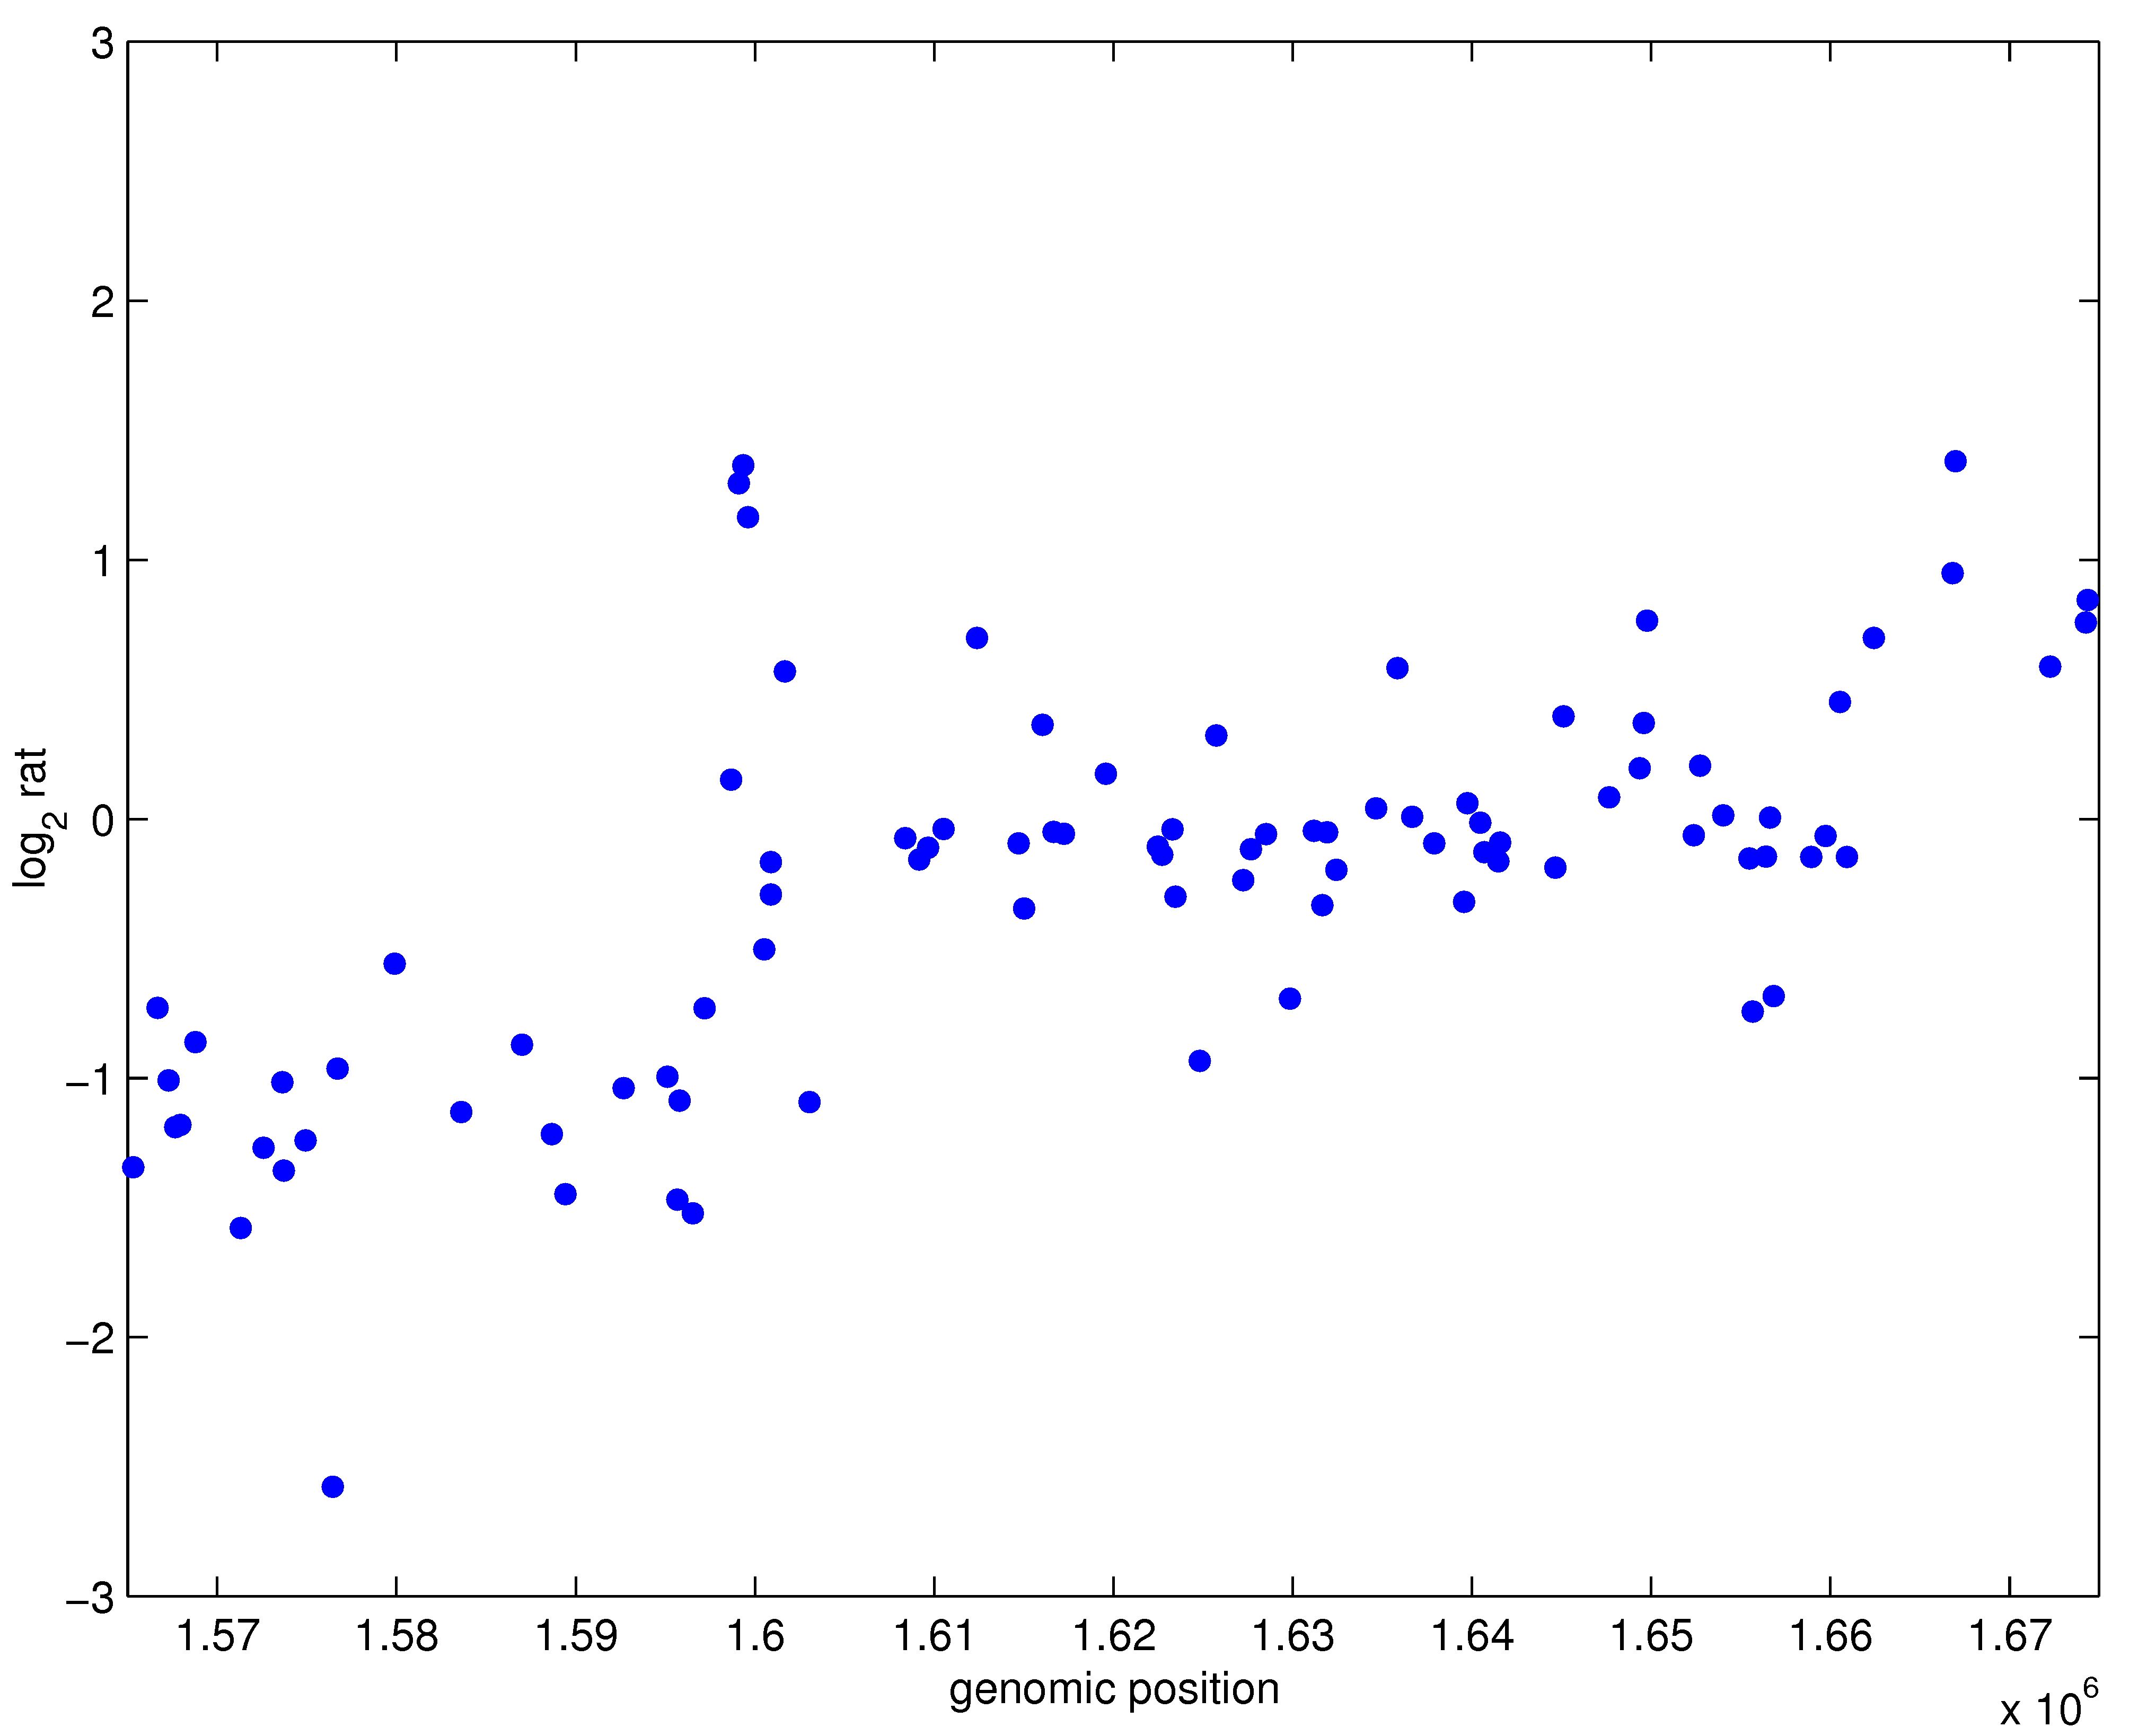
\epsfig{file = ../Figures/raw_profile_example.eps, clip=,
  bbllx=60, bblly=196, bburx=543, bbury=586}
$$
\centerline{
  A dot on the graph 
  $
  \displaystyle{
    = \log_2 \left\{ \frac{\text{ $\sharp$ copies of BAC(t) in the test
          genome }}{\text{$\sharp$ copies of BAC(t) in the reference
          genome}}\right\}}
  $
}

%%%%%%%%%%%%%%%%%%%%%%%%%%%%%%%%%%%%%%%%%%%%%%%%%%%%%%%%%%%%%
\newpage
\section{Interpretation of a CGH profile }
%%%%%%%%%%%%%%%%%%%%%%%%%%%%%%%%%%%%%%%%%%%%%%%%%%%%%%%%%%%%%
\vspace{-0.5cm}
$$
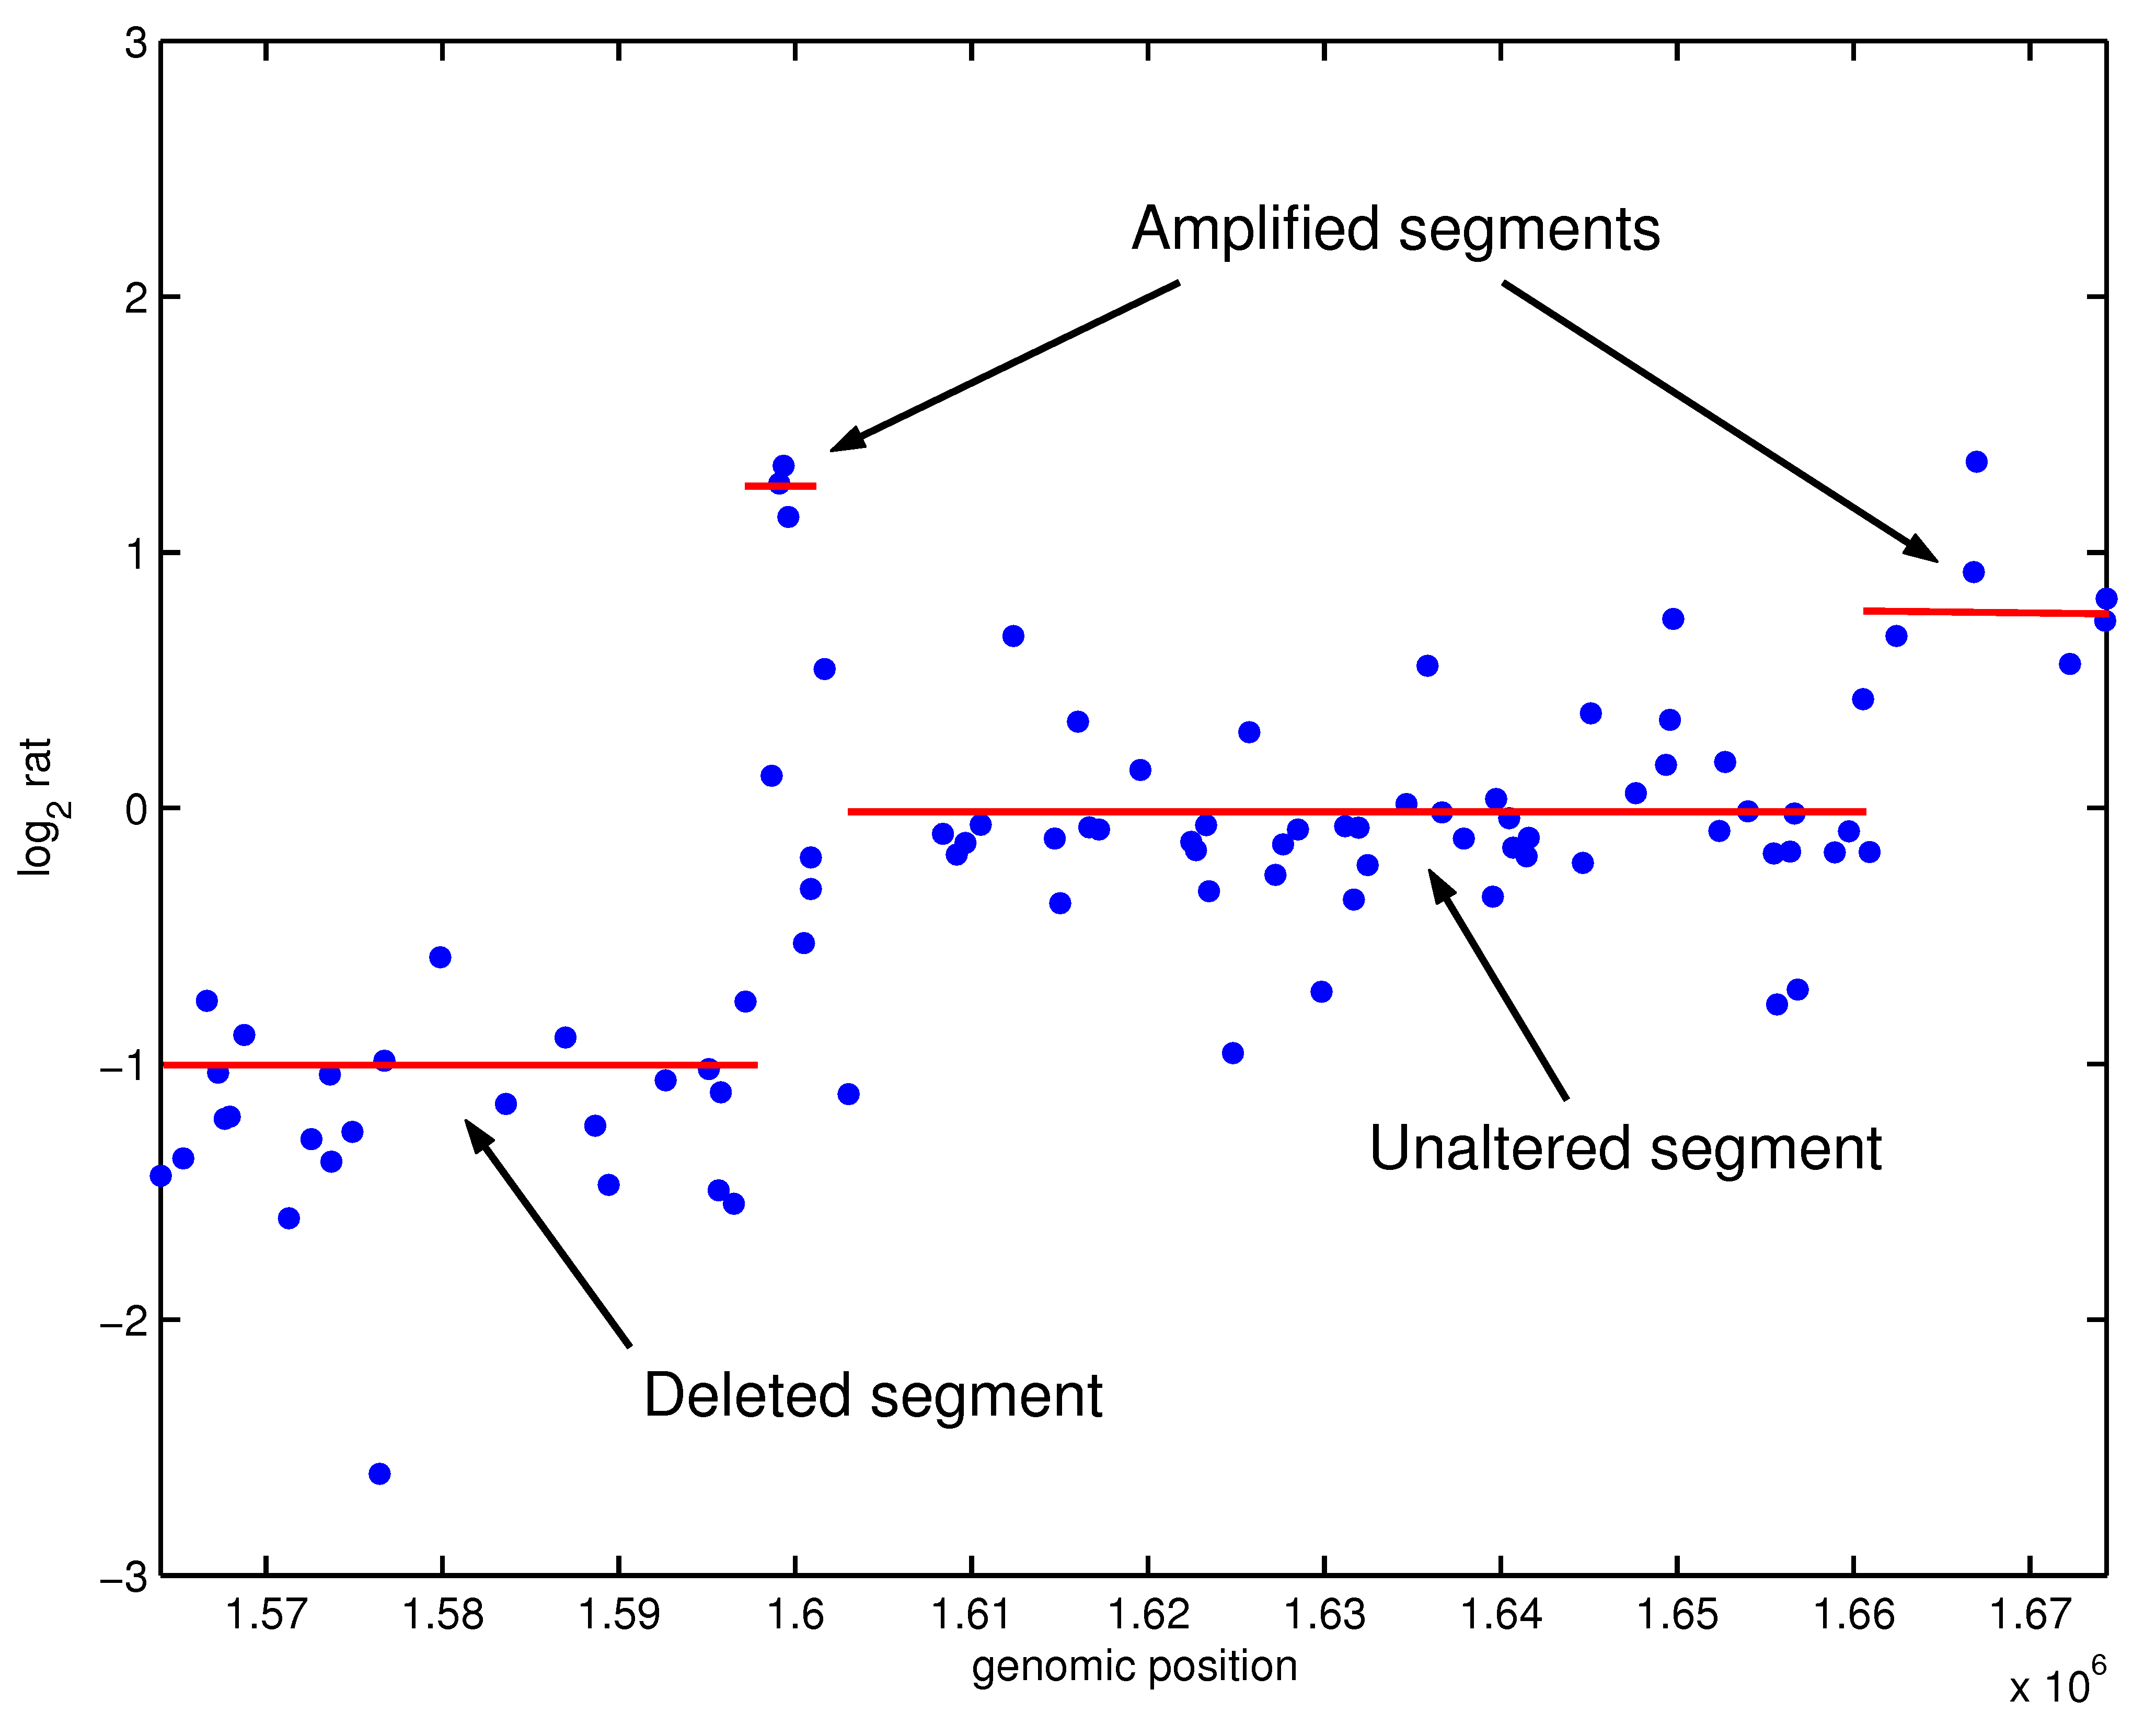
\epsfig{file = ../Figures/profile_example.eps, clip=,
  bbllx=60, bblly=196, bburx=543, bbury=586}
$$

%%%%%%%%%%%%%%%%%%%%%%%%%%%%%%%%%%%%%%%%%%%%%%%%%%%%%%%%%%
%%%%%%%%%%%%%%%%%%%%%%%%%%%%%%%%%%%%%%%%%%%%%%%%%%%%%%%%%%
\newpage
\chapter{A first modeling}
%%%%%%%%%%%%%%%%%%%%%%%%%%%%%%%%%%%%%%%%%%%%%%%%%%%%%%%%%%
%%%%%%%%%%%%%%%%%%%%%%%%%%%%%%%%%%%%%%%%%%%%%%%%%%%%%%%%%%

%%%%%%%%%%%%%%%%%%%%%%%%%%%%%%%%%%%%%%%%%%%%%%%%%%%%%%%%%%
\bigskip
\section{What to we have in mind?}
%%%%%%%%%%%%%%%%%%%%%%%%%%%%%%%%%%%%%%%%%%%%%%%%%%%%%%%%%%

\begin{itemize}
\item At position $t$, there exists a 'true' log-ratio $\lambda_t$,
  which depends on the relative copy number.
\item The value of the true log-ratio $\lambda_t$ is affected by
  abrupt changes:
                                %\vspace{-0.5cm}
  $$
  \epsfig{file = ../Figures/FigSeg_Intro.eps, clip=, bbllx=90,
    bblly=300, bburx=540, bbury=400, scale = 1.2}
  $$
  Position \paragraph{$t_1$, $t_2$, ..} are called {\sl
    breakpoints}. \paragraph{$\mu_k$} is the true log-ratio in segment
  \paragraph{$I_k$}.
\item The observed signal $Y_t$ is noisy:
  $$
  \mbox{for $t \in I_k$:} \qquad   Y_t = \mu_k + E_t.
  $$
\end{itemize}
%   where $\lambda_t$ is the true log-ratio 
%   and $E_t$ is a noise (typically, $E_t \sim \Ncal(0, \sigma^2)$).

%%%%%%%%%%%%%%%%%%%%%%%%%%%%%%%%%%%%%%%%%%%%%%%%%%%%%%%%%%
\newpage
\section{Statistical model} 
%%%%%%%%%%%%%%%%%%%%%%%%%%%%%%%%%%%%%%%%%%%%%%%%%%%%%%%%%%
\vspace{-0.5cm}\begin{itemize}
\item The breakpoints define a partition of the data into $K$
  segments of size $n_k$:
  $$
  I_k=\{t, t \in ]t_{k-1},t_k]\}, 
  \qquad
  Y^k=\{Y_t, t \in I_k\}.
  $$
\item Suppose that those parameters are constant between two changes:
  $$
  \mbox{if position $t$ is in segments $I_k$,} \qquad Y_t = \mu_k +
  E_t \sim \Ncal(\mu_k,\sigma_{(k)}^2).
  $$
\item The parameters of this model are: 
  $$
  T  =  (t_1, ..., t_{K-1}),
  \qquad
  \Theta  = (\theta_1,\hdots,\theta_K), \quad \theta_k=(\mu_k,\sigma_{(k)}^2).
  $$
\end{itemize}
Breakpoints detection aims at studying the \textblue{spatial structure
  of the signal}.

%%%%%%%%%%%%%%%%%%%%%%%%%%%%%%%%%%%%%%%%%%%%%%%%%%%%%%%%%%
\newpage
\subsection{Estimating the parameters}
%%%%%%%%%%%%%%%%%%%%%%%%%%%%%%%%%%%%%%%%%%%%%%%%%%%%%%%%%%

\paragraph{Log-Likelihood} (with a constant variance $\sigma^2$):
\begin{eqnarray*}
\Lcal_K(T, \Theta) & = & \sum_{k=1}^K \log \phi(\{Y_t\}_{t \in I_k};
\theta_k) \quad = \quad \sum_{k=1}^K \sum_{t \in I_k}\log \phi(Y_t; \theta_k) \\
& = & -n \log \sigma^2 - \frac1{\sigma^2} \sum_{k=1}^K \sum_{t \in
  I_k} (Y_t - \mu_k)^2 + \mbox{cst}. 
\end{eqnarray*}

\paragraph{2 important remarks:}
\begin{enumerate}
\item Because the data are supposed to be independent, the
  log-likelihood is a sum over all the segments.
\item Because the data are supposed to be Gaussian, maximum likelihood
  estimation is equivalent to least square fitting.
\end{enumerate}

%%%%%%%%%%%%%%%%%%%%%%%%%%%%%%%%%%%%%%%%%%%%%%%%%%%%%%%%%%
\newpage
\paragraph{When the breakpoints are known.}
Since we are in a Gaussian framework, maximum likelihood is equivalent
to least square estimate, so we get for the mean:
$$
\widehat{\mu}_k = \frac1{n_k} \sum_{t \in I_k} Y_t
$$
and for the variance,
\begin{itemize}
\item if it is supposed to be constant along the whole chromosome:
  $$
  \widehat{\sigma}^2 =  \frac1{n} \sum_{k=1}^K \sum_{t \in I_k} (Y_t -
  \widehat{\mu}_k)^2 
  $$
\item if it is supposed to be specific to each segment:
  $$
  \widehat{\sigma}^2_k = \frac1{n_k} \sum_{t \in I_k} (Y_t -
  \widehat{\mu}_k)^2 
  $$
\end{itemize}

%%%%%%%%%%%%%%%%%%%%%%%%%%%%%%%%%%%%%%%%%%%%%%%%%%%%%%%%%%
\newpage
\subsection{How to find the breakpoints?}

When $K$ is known , we have to minimize
$$
J_k(1, n) = \sum_{k=1}^K \sum_{t \in I_k} (Y_t - \widehat{\mu}_k)^2.
$$
\begin{itemize}
\item There are $\coefbin{n-1}{K-1}$ possible choices for the
  positions of the breakpoints $t_1, t_2, \dots, t_{K-1}$: \\
  \\
  \centerline{$\Rightarrow$ Impossible to explore for large
    $n$ and $K$}
\item $\sum_{t \in I_k} (Y_t - \widehat{\mu}_k)^2$ can be viewed as
  the 'cost' of segment $I_k$, i.e. the cost of putting data
  $Y_{t_{k-1}+1}$ to $Y_{t_{k+1}}$ in a single segment.
\item The optimization problem is actually a shortest path problem
  that can be solved thanks to \paragraph{dynamic programming}.
\end{itemize}

%%%%%%%%%%%%%%%%%%%%%%%%%%%%%%%%%%%%%%%%%%%%%%%%%%%%%%%%%%
\newpage
\paragraph{Dynamic programming.} Based on Bellmann's optimality
principle: \\
\\
\centerline{\sl Sub-paths of the optimal path are themselves optimal.}

\begin{description}
\item[Initialization:] For $0 \leq i < j \leq n$:
  $$
  J_1(i, j) = \sum_{t=i+1}^j (Y_t - \widehat{\mu})^2.
  $$
\item[Step $k$:] For $2 \leq k \leq K$:
  $$
  J_k(i, j) = \min_{i \leq h \leq j} \left[J_{k-1}(1, h) + J_1(h+1,
      j)\right].
  $$
  $J_k$ is called the \textblue{cost matrix}.
\end{description}

\paragraph{Remark:} Same principle as the Smith-Watermann algorithm
for sequence alignment.

%%%%%%%%%%%%%%%%%%%%%%%%%%%%%%%%%%%%%%%%%%%%%%%%%%%%%%%%%%
\newpage
\subsection{One last problem: the selection of $K$}

\noindent
\begin{tabular}{cc}
  \begin{tabular}{p{11cm}}
    \begin{itemize}
    \item The contrast $J_K$ necessarily decreases when the model
      becomes more complex. 
    \item The penalty function measures this complexity: $pen(K) = $
      $K+1$ with constant variance, $2K$ with heterogeneous variance.
    \item We look for the minimum of
      $$
      J_k + \beta pen(K)
      $$
      where $\beta$ is adaptively estimated (Lavielle(2003)).
    \end{itemize}
  \end{tabular}
  &
  \begin{tabular}{c}
    \epsfig{file = ../Figures/Select_K.ps, clip=, bbllx=146, bblly=529,
      bburx=464, bbury=777, width=12cm, height=12cm} 
  \end{tabular}
\end{tabular}

%%%%%%%%%%%%%%%%%%%%%%%%%%%%%%%%%%%%%%%%%%%%%%%%%%%%%%%%%%
\newpage
\section{Example of segmentation on array CGH data}
%%%%%%%%%%%%%%%%%%%%%%%%%%%%%%%%%%%%%%%%%%%%%%%%%%%%%%%%%%

\paragraph{Are the variances $\sigma^2_k$ homogeneous?} BT474 cell
line, chromosome 9: 
$$
\begin{tabular}{cc}
  Homogeneous variances & Heterogeneous variances \\
  \multicolumn{2}{c}{$K=4$ segments} \\
  \epsfig{file = ../Figures/bt474_c9_seg_homo_K4.eps, clip=, scale=0.7} &
  \epsfig{file = ../Figures/bt474_c9_seg_hetero_K4.eps, clip=, scale=0.7} \\
\end{tabular}
$$

%%%%%%%%%%%%%%%%%%%%%%%%%%%%%%%%%%%%%%%%%%%%%%%%%%%%%%%%%%
\newpage
\paragraph{Adaptive choice of the number of segments.} BT474 cell
line, chromosome 1:
$$
\begin{tabular}{cc}
  Homogeneous variances & Heterogeneous variances \\
  $\widehat{K} = 10$  segments & $\widehat{K} = 2$ segments \\
  \epsfig{file = ../Figures/bt474_c1_seg_homo_K10.eps, clip=, scale=0.7} &
  \epsfig{file = ../Figures/bt474_c1_seg_hetero_K2.eps, clip=, scale=0.7} \\
\end{tabular}
$$
Homogeneous variances result in smaller segments.

%%%%%%%%%%%%%%%%%%%%%%%%%%%%%%%%%%%%%%%%%%%%%%%%%%%%%%%%%%
\newpage
\subsection{Comparative study} 

\paragraph{Lai \& al. (Bioinformatics, 05).} On both synthetic and
real data (GBM brain tumor data), the methods performs well.
$$
%\epsfig{file = ../Figures/LPJ05-Fig1.eps, clip=, scale=1.2}
%\epsfig{file = ../Figures/LPJ05-Fig3.eps, clip=, scale=1.2}
\epsfig{file = ../Figures/LPJ05-Fig4.eps, clip=, scale=1.2}
$$


% %%%%%%%%%%%%%%%%%%%%%%%%%%%%%%%%%%%%%%%%%%%%%%%%%%%%%%%%%%
% \newpage
% \paragraph{ROC curves.} The sensitivity decreases for small segments
% when  signal-to-noise ratio (SNR) is small.
% $$
% \epsfig{file = ../Figures/LPJ05-Fig2.eps, clip=, scale=1.2}
% $$

%%%%%%%%%%%%%%%%%%%%%%%%%%%%%%%%%%%%%%%%%%%%%%%%%%%%%%%%%%
%%%%%%%%%%%%%%%%%%%%%%%%%%%%%%%%%%%%%%%%%%%%%%%%%%%%%%%%%%
\newpage
\chapter{A new model for segmentation-clustering}
%%%%%%%%%%%%%%%%%%%%%%%%%%%%%%%%%%%%%%%%%%%%%%%%%%%%%%%%%%
%%%%%%%%%%%%%%%%%%%%%%%%%%%%%%%%%%%%%%%%%%%%%%%%%%%%%%%%%%

\bigskip
\paragraph{Considering biologists objective and the need for a new
  model.}
$$
\begin{tabular}{cc}
  \epsfig{file = ../Figures/FigSegClas-1.eps, clip=, scale=0.7} &
  \epsfig{file = ../Figures/FigSegClas-2.eps, clip=, scale=0.7} \\
\end{tabular}
$$
We'd like segments of same type ('normal', 'deleted', amplified',
{\sl etc.}) to be gathered into groups.
% $$
% \epsfig{file = ../Figures/nouveau_modele.ps, angle=270, clip=,
%   bbllx=92, bblly=47, bburx=484, bbury=828, scale=0.9}
% $$

%%%%%%%%%%%%%%%%%%%%%%%%%%%%%%%%%%%%%%%%%%%%%%%%%%%%%%%%%%
\newpage
\begin{itemize}
\item We suppose there exists a \textblue{secondary underlying
    structure} of the segments into $P$ populations with weights
  $\pi_1,...,\pi_P (\sum_p \pi_p=1)$.
\item We introduce hidden variables, $Z_{kp}$ indicators of the
  population of origin of \textblue{segment $k$}.
\item Those variables are supposed independent, with multinomial
  distribution:
  $$
  \pi_p = \mbox{proportion of group $p$}
%   (Z_{k1},\hdots,Z_{kP}) \sim \mathcal{M}(1;\pi_1,\hdots,\pi_P).
  $$
\item Conditionally to the group to which the segment belongs, we know
  the distribution of $Y$:
  $$
  t \in I_k, k \in p \qquad \Rightarrow \qquad Y_t \sim \Ncal(m_p, s_p^2).
%   Y^k|Z_{kp}=1 \sim \Ncal({\bf 1}_{n_k} m_p, s_p^2 {\bf I}_{n_k}).
  $$
%\item It is a model of \textblue{segmentation/clustering}.
\item The parameters of this model are
  \begin{eqnarray*}
    \mbox{the brakpoint positions:} \quad T&=&(t_1, ..., t_{K-1}),\\
    \mbox{the mixture characteristics:} \quad \Theta&=&(\pi_1,\hdots,\pi_P;\theta_1,\hdots,\theta_P),    \quad  \text{where } \theta_p=(m_p,s_p^2).
  \end{eqnarray*}
\end{itemize}

%%%%%%%%%%%%%%%%%%%%%%%%%%%%%%%%%%%%%%%%%%%%%%%%%%%%%%%%%%
\newpage
\section{Likelihood and statistical units of the model }
%%%%%%%%%%%%%%%%%%%%%%%%%%%%%%%%%%%%%%%%%%%%%%%%%%%%%%%%%%

\paragraph{Mixture model of segments:} 
\vspace{-0.5cm}    \mbox{the brakpoint positions:} \quad 
\begin{itemize}
\item the statistical units are segments:$Y^k$,
\item the density of $Y^k$ is a mixture density:
  $$
  \log \Lcal_{KP}(T, \Theta)= \sum_{k=1}^K \log
  f_P(Y^k;\Theta)=\sum_{k=1}^K \log \left\{ \sum_{p=1}^P \pi_p
    \phi(Y^k;\theta_p) \right\}
  $$
\item \vspace{-0.5cm} If the $Y_ts$ are independent, we have:
  $$
  \log \Lcal_{KP}(T,\Theta) =\textcolor{red}{\sum_{k=1}^K} \log
  \left\{ \textcolor{blue}{\sum_{p=1}^P} \pi_p \textcolor{red}{\prod_{
        t \in I_k }}\phi(Y_t; \theta_p) \right\}. 
  $$
  instead of $ \log \Lcal_{P}(\Theta) =
  \textcolor{red}{\sum_{k=1}^K} \log \left\{ \textcolor{red}{\prod_{ t
        \in I_k }} \textcolor{blue}{\sum_{p=1}^P} \pi_p \phi(Y_t;
    \theta_p)\right \} $ in the classical mixture model where the
  statistical units are the elementary data $Y_t$s.
\end{itemize}

%%%%%%%%%%%%%%%%%%%%%%%%%%%%%%%%%%%%%%%%%%%%%%%%%%%%%%%%%%
\newpage
\section{An hybrid estimation algorithm}
%%%%%%%%%%%%%%%%%%%%%%%%%%%%%%%%%%%%%%%%%%%%%%%%%%%%%%%%%%

\paragraph{Alternate parameters estimation with $K$ and $P$ known}
\begin{enumerate}
\item When $T$ is fixed, the \textblue{Expectation-Maximisation (EM)}
  algorithm estimates $\Theta$:
  $$
  \hat{\Theta}^{(h+1)}=\underset{\Theta}{\arg\max} \left\{\log
    \Lcal_{KP}\left(\Theta,T^{(h)}\right) \right\}. 
  $$
  $$
  \log \Lcal_{KP}( \hat{\Theta}^{(h+1)}; \hat{T}^{(h)})
  \geq \log \Lcal_{KP}(\hat{\Theta}^{(h)};
  \hat{T}^{(h)})
  $$
\item When $\Theta$ is fixed, \textblue{dynamic programming} estimates $T$:
  $$
  \hat{T}^{(h+1)}=\underset{T}{\arg\max} \left\{\log
    \Lcal_{KP}\left(\hat{\Theta}^{(h+1)},T\right) \right\}. 
  $$
  $$
  \log \Lcal_{KP}(\hat{\Theta}^{(h+1)}; \hat{T}^{(h+1)})
  \geq \log \Lcal_{KP}(\hat{\Theta}^{(h+1)};
  \hat{T}^{(h)})
  $$
\end{enumerate} 
\paragraph{An increasing sequence  of likelihoods:}
$$\log \Lcal_{KP}(\hat{\Theta}^{(h+1)}; \hat{T}^{(h+1)}) \geq \log \Lcal_{KP}(\hat{\Theta}^{(h)}; \hat{T}^{(h)})$$

%%%%%%%%%%%%%%%%%%%%%%%%%%%%%%%%%%%%%%%%%%%%%%%%%%%%%%%%%%
\newpage
\subsection{EM algorithm: Prior and posterior probability}
%%%%%%%%%%%%%%%%%%%%%%%%%%%%%%%%%%%%%%%%%%%%%%%%%%%%%%%%%%
$$
  \begin{tabular}{cc}
    \textblue{Model:} & \textblue{Posterior probability:} \\
    \\
    $f(x) = \textred{\pi_1 f_1(x)} + \textgreen{\pi_2 f_2(x)} +
    \textblue{\pi_3 f_3(x)}$ & $\tau_{gk} = \Pr\{g \in f_k \;|\; x_g\}
    = \pi_k f_k(x_g) / f(x_g)$\\
    \\
    \epsfig{file=../Figures/Melange-densite.ps, height=6cm,
      width=12cm, bbllx=77, bblly=328, bburx=549, bbury=528, clip=}
    &
    \epsfig{file=../Figures/Melange-posteriori.ps, height=6cm, width=12cm,
      bbllx=83, bblly=320, bburx=549, bbury=537, clip=} 
  \end{tabular}
$$
$$  
\begin{array}{cccc}
  \quad \tau_{gk}~~(\%) \quad & \qquad g=1 \qquad & \qquad g=2 \qquad &
  \qquad g=3 \qquad \\
  \hline
  k = 1 & 65.8 & 0.7 & 0.0 \\
  k = 2 & 34.2 & 47.8 & 0.0 \\
  k = 3 & 0.0 & 51.5 & 1.0
\end{array}
$$

%%%%%%%%%%%%%%%%%%%%%%%%%%%%%%%%%%%%%%%%%%%%%%%%%%%%%%%%%%
\newpage
\subsection{Mixture model when the segmentation is known}
%%%%%%%%%%%%%%%%%%%%%%%%%%%%%%%%%%%%%%%%%%%%%%%%%%%%%%%%%%

\paragraph{Mixture model parameters estimators.}
\begin{eqnarray}
\mbox{posterior probability:} \qquad \hat{\tau}_{kp} & = & \frac{\hat{\pi}_p \phi(Y^k; \hat{\theta}_p)}{\suml \hat{\pi}_{h} \phi(Y^k; \hat{\theta}_{h})}. \nonumber
\end{eqnarray}
\begin{itemize}
\item the estimator the the mixing proportions is: $\hat{\pi}_p = \frac{\sumtau}{K}$.
\item In the gaussian case, $\theta_p=(m_p,s_p^2)$: 
\begin{eqnarray}
\mbox{weighted mean:} \qquad \hat{m}_p   &=&  \frac{\sumtau \sumt Y_t}{\sumtau n_k}, \nonumber \\
\mbox{weighted variance:} \qquad \hat{s}_p^2 &=&  \frac{\sumtau \sumt (Y_t- \hat{m}_p)^2}{\sumtau n_k}. \nonumber 
\end{eqnarray}
\item Big size vectors will have a bigger impact in the estimation of the parameters, via the term $\sumtau n_k$ \\
\end{itemize}

% %%%%%%%%%%%%%%%%%%%%%%%%%%%%%%%%%%%%%%%%%%%%%%%%%%%%%%%%%%
% \newpage
% \subsection{Segmentation with a fixed mixture}
% %%%%%%%%%%%%%%%%%%%%%%%%%%%%%%%%%%%%%%%%%%%%%%%%%%%%%%%%%%

% \paragraph{Back to dynamic programming}
% \begin{itemize}
% \item the incomplete mixture log-likelihood can be written as a sum of local log-likelihoods:
%   $$
%   \begin{array}{ccccc}
%     \Lcal_{KP}(T,\Theta) & = & \sumk f_P(Y^k;\Theta) 
%   \end{array}
%   $$
% \item the local log-likelihood of segment $k$ corresponds to the
%   mixture log-density of vector $Y^k$
%   $$
%   f_P(Y^k;\Theta)=\log \left\{\sum_{p=1}^P \pi_p \prod_{t \in
%       I_k} \phi(Y_t;\theta_p)\right\}.
%   $$
% \item $\log \Lcal_{KP}(T,\Theta)$ can be optimized in $T$ with $\Theta$ fixed, by dynamic programming. 
% \end{itemize}

% %%%%%%%%%%%%%%%%%%%%%%%%%%%%%%%%%%%%%%%%%%%%%%%%%%%%%%%%%%%
% \newpage
% \section{Model selection: $K=?$, $P=?$}
% %%%%%%%%%%%%%%%%%%%%%%%%%%%%%%%%%%%%%%%%%%%%%%%%%%%%%%%%%%%

% \subsection{Choosing the number of groups $P$} 

% \vspace{-0.5cm}
% We use the BIC criterion:
% $$
% BIC = \Lcal_{P} - \log n \times (\# \mbox{ of parameters}) / 2
% $$
% \vspace{-1cm}
% $$
% \begin{tabular}{cc}
%   Simulated sequence & $\Lcal_{KP}$ and $BIC$ criterion \\
%   \epsfig{file = ../Figures/Exemple_P2K4.eps, clip=, scale=0.7} &
%   \epsfig{file = ../Figures/Exemple_P2K4_BIC.eps, clip=, scale=0.7} \\
% \end{tabular}
% $$
% The log-likelihood $\Lcal$ (\textred{\bf ---}) always increases with
% $P$ while $BIC$ ({\bf ---}) has a maximum.

% %%%%%%%%%%%%%%%%%%%%%%%%%%%%%%%%%%%%%%%%%%%%%%%%%%%%%%%%%%%
% \newpage
% \subsection{Choosing the number of segments $K$} 

% The likelihood may decrease when $K$ increases:
% $$
% \begin{tabular}{lc}
%   \hspace{-1cm}
%   \begin{tabular}{l}
%     Simulated data: \\
%     \\
%     $f_2(Y^k;\Theta) =$ \\
%     \\
%     $0.5 \Ncal(0,1)+ 0.5 \Ncal(5,1)$ \\
%     \\
%     \\
%     Log-likelihood $\Lcal_{KP}$ \\
%     as a function of $K$ \\
%     \\
%     ($P=2$) \\
%     \\
%   \end{tabular}
%   & \begin{tabular}{c}
%     \epsfig{file = ../Figures/simulation_2.eps, clip=, scale=0.8}
%   \end{tabular}
% \end{tabular}
% $$
% $\rightarrow$ sort of self-penalization of the log-likelihood with
% respect to $K$.

%%%%%%%%%%%%%%%%%%%%%%%%%%%%%%%%%%%%%%%%%%%%%%%%%%%%%%%%%%%
\newpage
\section{Example: CGH for BT474 cell line}
%%%%%%%%%%%%%%%%%%%%%%%%%%%%%%%%%%%%%%%%%%%%%%%%%%%%%%%%%%%

\paragraph{Interest of clustering: an easy case.} Chromosome 9:
$$
  \begin{tabular}{cc}
    Segmentation & Segmentation/Clustering \\
    \multicolumn{2}{c}{$K=4$ segments} \\
    \epsfig{file = ../Figures/bt474_c9_seg_homo_K4, clip=, scale=0.7} 
    & 
    \epsfig{file = ../Figures/bt474_c9_segclas_homo_P3K4 , clip=, scale=0.7} 
  \end{tabular}
$$
Clustering defines 'deleted', 'normal' and 'amplified' groups.

\newpage

\paragraph{Interest of clustering: a more interesting case.}
Chromosome 1:
$$
\begin{tabular}{cc}
  Segmentation & Segmentation/Clustering \\
  $K=2$ & $P=3$, $K=8$ \\
  \epsfig{file = ../Figures/bt474_c1_seg_hetero_K2.eps, clip=, scale=0.7} 
  & \epsfig{file = ../Figures/resultat_P3K8.eps , clip=, scale=0.7} 
\end{tabular}
$$
Clustering detects an outliers and captures a 'normal' segment within
a large variance region.


% %%%%%%%%%%%%%%%%%%%%%%%%%%%%%%%%%%%%%%%%%%%%%%%%%%%%%%%%%%%
% %%%%%%%%%%%%%%%%%%%%%%%%%%%%%%%%%%%%%%%%%%%%%%%%%%%%%%%%%%%
% \newpage
% \chapter{Hidden Markov Model (HMM)}
% %%%%%%%%%%%%%%%%%%%%%%%%%%%%%%%%%%%%%%%%%%%%%%%%%%%%%%%%%%%
% %%%%%%%%%%%%%%%%%%%%%%%%%%%%%%%%%%%%%%%%%%%%%%%%%%%%%%%%%%%

% %%%%%%%%%%%%%%%%%%%%%%%%%%%%%%%%%%%%%%%%%%%%%%%%%%%%%%%%%%%
% \bigskip \bigskip 
% \section{Statistical model}
% %%%%%%%%%%%%%%%%%%%%%%%%%%%%%%%%%%%%%%%%%%%%%%%%%%%%%%%%%%%

% \paragraph{Alternative modeling.}
% Each position $t$, has an unknown label $Z_t$
% revealing the status of the position:
% $$
% Z_t \in \{1, 2, \dots, P\}.
% $$
% Given the $Z_t$s, the observed data $Y_t$s are independent with
% Gaussian distribution:
% $$
% \{Y_t \;|\; Z_t = p\} \sim \Ncal(m_p, s_p^2).
% $$

% \paragraph{Spatial structure.}
% The process $Z_t$ is a Markov chain with transition matrix $\Pibf$:
% $$
% \Pibf = \left(
%   \begin{array}{cccc}
%     \pi(1, 1) & \pi(1, 2) & \dots & \pi(1, P) \\ 
%     \pi(2, 1) & \pi(2, 2) & \dots & \pi(2, P) \\ 
%     \vdots & \vdots & & \vdots \\
%     \pi(P, 1) & \pi(P, 2) & \dots & \pi(P, P) \\ 
%   \end{array}
% \right).
% $$

% %%%%%%%%%%%%%%%%%%%%%%%%%%%%%%%%%%%%%%%%%%%%%%%%%%%%%%%%%%%
% \newpage
% \paragraph{Hidden structure.}
% Because the breakpoints are expected to be rare, the self transition
% probabilities should be close to 1:
% $$
% \pi(p, p) = 1 - \varepsilon_p.
% $$
% The Markov chain $\{Z_t\}$ rarely jumps from one step to another.

% \paragraph{Length of the segments.}
% The general properties of Markov chains implies that the sojourn time
% in each state, i.e. the length of the segments, has a geometric
% distribution:
% $$
% \mbox{if } I_k \in p, 
% \qquad (T_k - T_{k-1}) \sim \Gcal(1-\varepsilon_p), 
% \qquad \Esp(T_k -T_{k-1}) = \frac1{\varepsilon_p}.
% $$
% In the case of CGH, nothing supports this hypothesis. \\
% In the case of other chromosomic chips...?

% %%%%%%%%%%%%%%%%%%%%%%%%%%%%%%%%%%%%%%%%%%%%%%%%%%%%%%%%%%%
% \newpage
% \paragraph{ BT474 cell line, chromosome 9:}
% $$
% \begin{tabular}{cc}
%   Segmentation / Clustering & HMM (forward/backward) \\
%   \\
%   \epsfig{file = ../Figures/Comp_HMM_SegClus.ps, clip=, bbllx=148,
%     bblly=480, bburx=464, bbury=717, width=12cm, height=10cm} 
%   &
%   \epsfig{file = ../Figures/Comp_HMM_SegClus.ps, clip=, bbllx=148,
%     bblly=227, bburx=464, bbury=464, width=12cm, height=10cm} \\
%   4 segments & 24 segments 
% \end{tabular}
% $$

% %%%%%%%%%%%%%%%%%%%%%%%%%%%%%%%%%%%%%%%%%%%%%%%%%%%%%%%%%%%
% %%%%%%%%%%%%%%%%%%%%%%%%%%%%%%%%%%%%%%%%%%%%%%%%%%%%%%%%%%%
% \newpage
% \chapter{Conclusion and future works}
% %%%%%%%%%%%%%%%%%%%%%%%%%%%%%%%%%%%%%%%%%%%%%%%%%%%%%%%%%%%
% %%%%%%%%%%%%%%%%%%%%%%%%%%%%%%%%%%%%%%%%%%%%%%%%%%%%%%%%%%%

% \paragraph{What we did:}
% \vspace{-0.5cm}
% \begin{itemize}
% \item Definition of a new model that considers the \textit{a priori}
%   knowledge we have about the biological phenomena under study.
% \item Development of an hybrid algorithm (EM/dynamic programming) for
%   the parameters estimation (problems linked to EM: initializtion,
%   local maxima, degeneracy).
% \item Still waiting for an other data set to assess the performance of
%   the clustering.
% \end{itemize}

% \paragraph{What we still have to do:}
% \vspace{-0.5cm}
% \begin{itemize}
% \item Modeling: Comparison with Hidden Markov Models
% \item Model choice: Develop an adaptive procedure for two components.
% \item Other application field: DNA sequences (in progress)
% \end{itemize}

% %%%%%%%%%%%%%%%%%%%%%%%%%%%%%%%%%%%%%%%%%%%%%%%%%%%%%%%%%%%
% \newpage
% %%%%%%%%%%%%%%%%%%%%%%%%%%%%%%%%%%%%%%%%%%%%%%%%%%%%%%%%%%%
% %%%%%%%%%%%%%%%%%%%%%%%%%%%%%%%%%%%%%%%%%%%%%%%%%%%%%%%%%%%
% \newpage
% \chapter{Additional slides}
% %%%%%%%%%%%%%%%%%%%%%%%%%%%%%%%%%%%%%%%%%%%%%%%%%%%%%%%%%%%
% %%%%%%%%%%%%%%%%%%%%%%%%%%%%%%%%%%%%%%%%%%%%%%%%%%%%%%%%%%%

% %%%%%%%%%%%%%%%%%%%%%%%%%%%%%%%%%%%%%%%%%%%%%%%%%%%%%%%%%%
% \newpage
% \section{Influence of the vectors size on the affectation (MAP)}
% %%%%%%%%%%%%%%%%%%%%%%%%%%%%%%%%%%%%%%%%%%%%%%%%%%%%%%%%%%

% \begin{itemize}
% \item The density of $Y^k$ can be written as follows:
%   $$
%   \phi(Y^k;\theta_p) = \exp \left\{ -\frac{n_k}{2} \left( \log(2 \pi
%       s_p^2) + \frac{1}{s_p^2} \left[ (\bar{y_k^2}- \bar{y}_k^2) +
%         (\bar{y}_k-m_p)^2 \right]\right)\right\}
%   $$
%   $(\bar{y}_k-m_p)^2$: distance of the mean of vector $k$ to
%   population $p$ \\
%   \\
%   $(\bar{y_k^2}- \bar{y}_k^2)$: intra-vector $k$ variability \\
% \item Big size Individuals will be affected with certitude to the
%   closest population 
%   $$
%   \begin{array}{ccc|ccc}
%     \underset{n_k \to \infty}{\lim} \tau_{kp_0}  &=& 1   &
%     \underset{n_k \to \infty}{\lim} \tau_{kp} &=&  0  \\ 
%     \underset{n_k \to 0}{\lim} \tau_{kp_0} & = &\pi_{p_0} &
%     \underset{n_k \to 0}{\lim} \tau_{kp} &= & \pi_p  
%   \end{array}
%   $$
% \end{itemize}

% %%%%%%%%%%%%%%%%%%%%%%%%%%%%%%%%%%%%%%%%%%%%%%%%%%%%%%%%%%%
% \newpage
% \section{Non increasing likelihood}

% \bigskip
% \paragraph{What is going on?}
% $$
% \epsfig{file = ../Figures/segmentation_melange_simulation_2.eps,
%   clip=, scale=0.85} 
% $$
% When the true number of segments is reached (6), segments are cut on
% the edges. 

% %%%%%%%%%%%%%%%%%%%%%%%%%%%%%%%%%%%%%%%%%%%%%%%%%%%%%%%%%%%
% \newpage
% \subsection{Explaining the behavior of the likelihood}
% %%%%%%%%%%%%%%%%%%%%%%%%%%%%%%%%%%%%%%%%%%%%%%%%%%%%%%%%%%%

% \paragraph{Optimization of the incomplete likelihood with dynamic programming:}
% \begin{eqnarray*}
% \log \Lcal_{KP}(T;\Theta)&=& Q_{KP}(T;\Theta)-H_{KP}(T;\Theta)\\ 
% Q_{KP}(T;\Theta) &=& \sum_k \sum_p \tau_{kp} \log (\pi_p) + \sum_k \sum_p \tau_{kp} \log \phi(Y^k; \theta_p) \\
% H_{KP}(T;\Theta) &=& \sum_k \sum_p \tau_{kp} \log \tau_{kp} 
% \end{eqnarray*}
% \paragraph{Hypothesis:}
% \begin{enumerate}
% \item We suppose that the true number of segments is $K^*$ and that
%   the partitions are nested for $K \geq K^*$.  Segment $Y^K$ is cut
%   into $(Y_1^K,Y_2^K)$: 
%   $$
%   \phi(Y^{K};\theta_p)=\phi(Y_1^{K};\theta_p) \times
%   \phi(Y_2^{K};\theta_p).
%   $$
% \item We suppose that if $Y^{K} \in p$ then $(Y_1^{K},Y_2^{K}) \in p$: $$\tau_{p}(Y^K) \simeq \tau_{p}(Y_1^K) \simeq \tau_{p}(Y_2^K) \simeq \tau_p.$$
% \end{enumerate}
% %and $\hat{\pi}_p=\sum_k \hat{\tau}_{kp}/K$.

% %%%%%%%%%%%%%%%%%%%%%%%%%%%%%%%%%%%%%%%%%%%%%%%%%%%%%%%%%%%
% \newpage
% \subsection{An intrinsic penality}
% %%%%%%%%%%%%%%%%%%%%%%%%%%%%%%%%%%%%%%%%%%%%%%%%%%%%%%%%%%%

% \paragraph{Under hypothesis 1-2:}
% $$\forall K\geq K^*, \log \hat{\Lcal}_{(K+1),P}-\log \hat{\Lcal}_{(K),P}\simeq \sum_p \hat{\pi}_p \log (\hat{\pi}_p) - \sum_p \hat{\tau}_p \log (\hat{\tau}_p)\leq 0$$

% \paragraph{The log-likelihood is decomposed into two terms\rm }
% \begin{itemize}
% \item A term of \textblue{fit} that increases with $K$, and is constant from a certain $K^*$ (nested partitions) $$\sum_k \sum_p \hat{\tau}_{kp} \log \phi(Y^k; \hat{\theta}_p).$$ \\
% \item A term of \textblue{differences of entropies} that decreases with $K$: plays the role of penalty for the choice of $K$
% $$K\sum_p \hat{\pi}_p \log (\hat{\pi}_p) - \sum_k \sum_p \hat{\tau}_{kp} \log \hat{\tau}_{kp}.$$
% \end{itemize}

% % \begin{center}  {Choosing the number of segments $K$ when $P$ is fixed can be done with a penalized likelihood} \end{center}

% %%%%%%%%%%%%%%%%%%%%%%%%%%%%%%%%%%%%%%%%%%%%%%%%%%%%%%%%%%%
% \newpage
% \paragraph{Incomplete Likelihood behavior with respect to the number of
%   segments } 
% %%%%%%%%%%%%%%%%%%%%%%%%%%%%%%%%%%%%%%%%%%%%%%%%%%%%%%%%%%%
% %\vspace{-1cm}
% $$
% \epsfig{file = ../Figures/vrais_Pfixe.eps, clip=, scale=0.8}
% %  bbllx=0, bblly=41, bburx=700, bbury=478}
% $$

% The incomplete log-likelihood is decreasing from de $K=8$:
% $$\hat{\Lcal}_{KP}(\hat{T};\hat{\Theta})=\sum_k \log \left\{
%   \sum_p \hat{\pi}_p \phi(Y^k;\hat{\theta}_p)\right\}.
% $$ 

% %%%%%%%%%%%%%%%%%%%%%%%%%%%%%%%%%%%%%%%%%%%%%%%%%%%%%%%%%%%
% \newpage
% \paragraph{Decomposition of the log-likelihood.}
% %%%%%%%%%%%%%%%%%%%%%%%%%%%%%%%%%%%%%%%%%%%%%%%%%%%%%%%%%%%
% \vspace{-1cm}
% $$
%   \begin{tabular}{cc}
%     term of fit & differences of entropies \\
%     \epsfig{file = ../Figures/vrais_class_Pfixe.eps, clip=,
%     scale=0.7} 
%     & 
%     \epsfig{file = ../Figures/diff_entropie.eps, clip=,
%     scale=0.7} \\
%     $\sum_k \sum_p \hat{\tau}_{kp} \log \phi(Y^k;\hat{\theta}_p)$ &
%     $K\sum_p \hat{\pi}_p \log (\hat{\pi}_p) - \sum_k \sum_p
%     \hat{\tau}_{kp} \log \hat{\tau}_{kp}$ 
%   \end{tabular}
% $$
% The term of fit is "constant" from $K=8$: 
% $$
% Q_{KP}(T;\Theta)=K \sum_p \pi_p \log{\pi_p}+ \sum_k \sum_p \tau_{kp}
% \log \phi( Y^k;\theta_p).
% $$

%%%%%%%%%%%%%%%%%%%%%%%%%%%%%%%%%%%%%%%%%%%%%%%%%%%%%%%%%%%%%
%%%%%%%%%%%%%%%%%%%%%%%%%%%%%%%%%%%%%%%%%%%%%%%%%%%%%%%%%%%%%
\newpage
\chapter{Multiple arrays analysis}
%%%%%%%%%%%%%%%%%%%%%%%%%%%%%%%%%%%%%%%%%%%%%%%%%%%%%%%%%%%%%
%%%%%%%%%%%%%%%%%%%%%%%%%%%%%%%%%%%%%%%%%%%%%%%%%%%%%%%%%%%%%

\subsection{Two examples.}

\paragraph{1 - Comparing {\sl A. Thaliana} mutants or ecotypes.}
Chromosomal rearrangement can be detected by comparing CGH profiles
observed on individual from different genotypes.

\paragraph{2 - Comparing groups of patients.}
To detect chromosomal aberration associated with a specific disease
(e.g. breast cancer), we analyse the profiles of several ill patients
jointly.

\bigskip\bigskip
\subsection{First approach: Common breakpoints.}

Assuming that all the patients of the same group have their
breakpoints at the same positions, leads to \emphase{segment a
  multivariate signal}, which can be achieved using DP.

This is doable but \emphase{biologically irrelevant}.

%%%%%%%%%%%%%%%%%%%%%%%%%%%%%%%%%%%%%%%%%%%%%%%%%%%%%%%%%%
\newpage
\subsection{Breast cancer dataset (Inst. Curie): Chromosome 8.} \\
\\
\begin{tabular}{ccc}
  & Good prognosis (53 patients) & Bad prognosis (81 patients) \\
  \hspace{-1cm}
  \begin{tabular}{p{2.5cm}} Number of breakpoints \end{tabular} &
  \begin{tabular}{c}
    \epsfig{file =
      /RECHERCHE/RUPTURES/Exposes/Figures/CurieChromo8Gp1_K.eps, clip=,
      width=10cm, height=6cm}
  \end{tabular} 
  &
  \begin{tabular}{c}
    \epsfig{file =
      /RECHERCHE/RUPTURES/Exposes/Figures/CurieChromo8Gp2_K.eps, clip=,
      width=10cm, height=6cm} 
  \end{tabular} \\
  \hspace{-1cm}
  \begin{tabular}{p{2.5cm}} Position of the breakpoints \end{tabular} &
  \begin{tabular}{c}
    \epsfig{file =
      /RECHERCHE/RUPTURES/Exposes/Figures/CurieChromo8Gp1_T.eps, clip=,
      width=10cm}
  \end{tabular} 
  &
  \begin{tabular}{c}
    \epsfig{file =
      /RECHERCHE/RUPTURES/Exposes/Figures/CurieChromo8Gp2_T.eps, clip=,
      width=10cm}
  \end{tabular} 
\end{tabular}

%%%%%%%%%%%%%%%%%%%%%%%%%%%%%%%%%%%%%%%%%%%%%%%%%%%%%%%%%%%%%
\newpage
\section{Correlated profiles}
%%%%%%%%%%%%%%%%%%%%%%%%%%%%%%%%%%%%%%%%%%%%%%%%%%%%%%%%%%%%%

\hspace{-2cm}
\begin{tabular}{cc}
  \begin{tabular}{p{12cm}}
    We want to account for \emphase{correlations between profiles}. \\ \\
    \emphase{Different probe affinities} may alter all the profiles at the same
    position. \\ \\
    Denoting $Y_{it}$ the profile of patient $i$ at position $t$
    (belonging to segment $I_{ik}$), we
    set
    $$
    Y_{it} = \mu_{ik} + U_t + E_{it}
    $$
    where $\mu_{ik}$ is the mean of segment $I_{ik}$ and
    \emphase{$U_t$ is the random effect of probe $t$}: 
    $$
    \{E_{it}\} \mbox{ iid } \Ncal(0, \sigma^2),  
    \quad
    \{U_t\} \mbox{ iid } \Ncal(0, \gamma^2).  
    $$
  \end{tabular}
  &
  \begin{tabular}{l}
    \epsfig{file = ../Figures/nakao-mat.txt-MixSeg.eps, width=11cm,
    height=14cm, bbllx=90, bblly=220, bburx=380, bbury=590, clip=}
  \end{tabular}
\end{tabular}

% %%%%%%%%%%%%%%%%%%%%%%%%%%%%%%%%%%%%%%%%%%%%%%%%%%%%%%%%%%%%%
% \newpage
% \section{Mixed segmentation model}
% %%%%%%%%%%%%%%%%%%%%%%%%%%%%%%%%%%%%%%%%%%%%%%%%%%%%%%%%%%%%%

% \paragraph{Covariance between profiles.}
% $$
% \Cov(Y_{it}, Y_{i't'}) = \Cov(U_t + E_{it}, U_{t'} + E_{i't'}) = 
% \left\{
%   \begin{array}{cl}
%     \gamma^2 & \mbox{if } t = t' \\
%     0 & \mbox{otherwise}
%   \end{array}.
% \right.
% $$

% \paragraph{Matrix form.}
% We end up with a mixed linear model with a segmentation term ($\Tbf$):
% $$
% \Ybf = \Tbf \mubf + \Zbf \Ubf + \Ebf
% $$
% where
% \begin{itemize}
% \item \vspace{-0.5cm} $m$ is the number of patients, $n$ is the length
%   of each profile
% \item \vspace{-0.5cm} $\Zbf$ is the ($nm \times n$) \emphase{design
%     matrix} that gives the probe corresponding to each data point.
% \item \vspace{-0.5cm} $\Ubf$ is the $n$-vector containing the random
%   effects of the probes.
% \end{itemize}
% \vspace{-0.5cm} \refer{Lebarbier et al.}{2007}

%%%%%%%%%%%%%%%%%%%%%%%%%%%%%%%%%%%%%%%%%%%%%%%%%%%%%%%%%%
\newpage
\section{Estimation of the parameters}
%%%%%%%%%%%%%%%%%%%%%%%%%%%%%%%%%%%%%%%%%%%%%%%%%%%%%%%%%%

\paragraph{Direct maximisation.}
Due to correlations, the variance is not diagonal, so the
log-likelihood is not additive anymore $\Rightarrow$ \emphase{No
  dynamic programming}

\subsection{A second  DP-EM algorithm} 

\vspace{-0.5cm} 
The \emphase{conditional variance} of the $Y_{it}$ given $U$ is
diagonal, so DP can be used to estimate the breakpoints  given $U$.
% $\Ubf$ is seen as an unobserved. \refer{Foulley}{Lecture notes}

\paragraph{E step.} Calculate the conditional moments of the random
effect given the data:
$$
\widehat{\Esp}(U_t|Y_{it}), \qquad \widehat{\Var}(U_t|Y_{it}).
$$
\paragraph{M step.} Denoting $\widehat{U_t} = 
\widehat{\Esp}(U_t|Y_{it})$ , perform the segmentation as follows.
% :
% $$
% \widehat{\Tbf \mubf} = \arg\min_{\Tbf\mubf} \|\Ybf -
% {\Tbf\mubf}-\Zbf \widehat{\Ubf}\|^2.
% $$

\noindent A \emphase{two-stage dynamic programming} is required to
achieve this step for numerous patients. \refer{Picard et al.}{?}

% %%%%%%%%%%%%%%%%%%%%%%%%%%%%%%%%%%%%%%%%%%%%%%%%%%%%%%%%%%
% \newpage
% \section{Nakao data, chromosome 20}
% %%%%%%%%%%%%%%%%%%%%%%%%%%%%%%%%%%%%%%%%%%%%%%%%%%%%%%%%%%

% The random effect has an influence on the detected breakpoints. 

% \noindent
% \begin{tabular}{cc}
%   \begin{tabular}{p{10cm}}
%     We find a \emphase{large negative random effect} $U_t$ has at position
%     37. \\ \\
%     $\rightarrow$ poor probe affinity or wrong annotation.
%   \end{tabular}
%   &
%   \begin{tabular}{l}
%     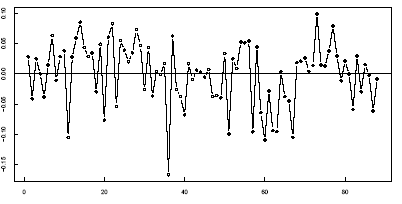
\epsfig{file= ../FIGURES/Group1_U.ps, width=12cm, height=6cm,
%     bbllx=38, bblly=49, bburx=562, bbury=293, clip=}
%   \end{tabular} \\
%   \begin{tabular}{p{10cm}}
%     Comparison \textred{individual} / multiple segmentation. \\
%     \\
%     The breakpoints detected around position 37 vanish.
%   \end{tabular}
%   &
%   \begin{tabular}{l}
%     \epsfig{file= ../FIGURES/Exemple_profile6_group1.ps, width=12cm,
%     height=6cm, bbllx=65, bblly=65, bburx=560, bbury=182, clip=} 
%   \end{tabular}
% \end{tabular}

%%%%%%%%%%%%%%%%%%%%%%%%%%%%%%%%%%%%%%%%%%%%%%%%%%%%%%%%%%
\newpage
\section{Bladder cancer data (Inst. Curie, F. Radvanyi)}
%%%%%%%%%%%%%%%%%%%%%%%%%%%%%%%%%%%%%%%%%%%%%%%%%%%%%%%%%%

\noindent
\begin{tabular}{cc}
  \begin{tabular}{p{10cm}}
    \paragraph{Global analysis} \\ \\
    We find a \emphase{large positive random effect} $U_t$ has at position
    87. \\ \\
    $\rightarrow$ poor probe affinity or wrong annotation.
  \end{tabular}
  &
  \begin{tabular}{c}
    \epsfig{file= ../FIGURES/Random_Effect.ps, clip, width=7cm,
    height=12cm, angle=270}
  %, bbllx=100, bblly=60, bburx=510, bbury=780}
  \end{tabular} \\
  \begin{tabular}{p{10cm}}
    The mean profile of the whole set of patients can be corrected
    from the probe effect: \\
    (${\bf \cdots}$) mean of raw profiles, \\
    (${\bf \circ}$) mean of corrected profiles
  \end{tabular}
  &
  \begin{tabular}{c}
    \epsfig{file= ../FIGURES/Graphe_Profils_Moyens_Segmentes.ps, clip,
    width=7cm, height=12cm, angle=270}
  \end{tabular}
\end{tabular}

%%%%%%%%%%%%%%%%%%%%%%%%%%%%%%%%%%%%%%%%%%%%%%%%%%%%%%%%%%
\newpage
\noindent
\begin{tabular}{cc}
  \begin{tabular}{p{10cm}}
    \paragraph{Individual profiles.}
    The random effect has an influence on the segmentation. \\
    \begin{itemize}
    \item Breakpoints around position 86 are detected in individual
      profiles when analysed independently (\textred{--}).
    \item They vanish after correction of the probe effect vanish
      ({\bf --}).
    \end{itemize}
  \end{tabular}
  &
  \begin{tabular}{c}
    \epsfig{file= ../FIGURES/Profils2_9_29.ps, width=12cm,
    height=16cm, clip=} 
  \end{tabular}
\end{tabular}

%%%%%%%%%%%%%%%%%%%%%%%%%%%%%%%%%%%%%%%%%%%%%%%%%%%%%%%%%%%%%
%%%%%%%%%%%%%%%%%%%%%%%%%%%%%%%%%%%%%%%%%%%%%%%%%%%%%%%%%%%%%
\newpage
\chapter{Looking for common aberrations}
%%%%%%%%%%%%%%%%%%%%%%%%%%%%%%%%%%%%%%%%%%%%%%%%%%%%%%%%%%%%%
%%%%%%%%%%%%%%%%%%%%%%%%%%%%%%%%%%%%%%%%%%%%%%%%%%%%%%%%%%%%%

\noindent
\begin{tabular}{cc}
  \begin{tabular}{p{7.5cm}}
    To detect \emphase{aberrations associated to a disease}
    (e.g. bladder cancer), we look for aberrations that appear
    \emphase{'significantly'  often} among a set of patients.  \\ \\
  $X_{it}$ denotes the status of position $t$ for patient $i$:
  $$
  \begin{tabular}{rcrl}
    $X_{it}$ & = & \textblue{--1} & \textblue{(loss)} \\
    & = & 0 & (normal) \\
    & = & \textred{+1} & \textred{(gain)}
  \end{tabular}
  $$
  \refer{Hupp� et al.}{2004}
  \end{tabular}
  &
  \begin{tabular}{c}
    \epsfig{file=/RECHERCHE/RUPTURES/Etudes/Curie/MinRegion/Data1/Profiles.eps,
    }
  \end{tabular}
\end{tabular}

% %%%%%%%%%%%%%%%%%%%%%%%%%%%%%%%%%%%%%%%%%%%%%%%%%%%%%%%%%%%%%%%%%%%%%%
% \newpage
% \section{Discretized CGH profiles}
% %%%%%%%%%%%%%%%%%%%%%%%%%%%%%%%%%%%%%%%%%%%%%%%%%%%%%%%%%%%%%%%%%%%%%%

% \hspace{-2cm}
% \begin{tabular}{cc}
%   \begin{tabular}{p{7cm}}
%     $i = 1..m$ patients \\
%     ($m = 84$), \\
%     \\
%     $t = 1..n$ positions \\
%     ($n = 2360$) \\
%     \\
%     $X_{it}$ = status of\\
%     patient $i$ %\\
%     at position $t$. \\
%     \\
%     \begin{tabular}{rcrl}
%       $X_{it}$ & = & \textblue{--1} & \textblue{(loss)} \\
%        & = & 0 & (normal) \\
%        & = & \textred{+1} & \textred{(gain)}
%     \end{tabular}
%   \end{tabular}
%   &
%   \begin{tabular}{c}
%     \epsfig{file=/RECHERCHE/RUPTURES/Etudes/Curie/MinRegion/Data1/Profiles.eps}
%   \end{tabular}
% \end{tabular}

%%%%%%%%%%%%%%%%%%%%%%%%%%%%%%%%%%%%%%%%%%%%%%%%%%%%%%%%%%%%%%%%%%%%%%
\newpage
\section{Minimal region}
%%%%%%%%%%%%%%%%%%%%%%%%%%%%%%%%%%%%%%%%%%%%%%%%%%%%%%%%%%%%%%%%%%%%%%

\begin{tabular}{cc}
  \begin{tabular}{p{15cm}}
    A minimal region is a sequence of \emphase{successive positions}
    for which the \emphase{same status} is observed in \emphase{large
    number} of patients at the same time. \refer{Rouveirol \& al.}{2006}\\
    \\
    \paragraph{Data.} $M^* = 31$ patients present $\ell =
    5$ successive deletions between positions 1189 and 1193, in
    chromosome 9. \\
    \\
    \paragraph{Question.} Is this significant, given the number of
    patients ($m=84$) and the profiles length ($n=2340$)?
%     It is characterized by
%     \begin{itemize}
%     \item its position $t^* \in \{1..n\}$, 
%     \item its length $\ell$,
%     \item its status $s \in \{-1, 0, +1\}$, 
%     \item the number of patients $M^* \in \{1..m\}$.
%     \end{itemize} \\
  \end{tabular}
  &
  \begin{tabular}{c}
    \epsfig{file=/RECHERCHE/RUPTURES/Etudes/Curie/MinRegion/Data1/ExMinRegion.eps,
      clip=, bbllx=270, bblly=209, bburx=400, bbury=593}
  \end{tabular}
\end{tabular}


%%%%%%%%%%%%%%%%%%%%%%%%%%%%%%%%%%%%%%%%%%%%%%%%%%%%%%%%%%%%%%%%%%%%%%
\newpage
\section{Motif Statistics}
%%%%%%%%%%%%%%%%%%%%%%%%%%%%%%%%%%%%%%%%%%%%%%%%%%%%%%%%%%%%%%%%%%%%%%

\paragraph{Binary case.} Assume that only 2 status exist: 
$$
X_{it} = \left\{ 
  \begin{array}{rl}
    1 & \mbox{for aberration,} \\
    0 & \mbox{for normal.}
  \end{array}
\right.
$$

\paragraph{Region.} A minimal region is then a $\ell$-run of
1s. Denote
$$
Y_{it} = \prod_{u=t-\ell+1}^t X_{it} = \left\{ 
  \begin{array}{rl}
    1 & \mbox{if a $\ell$-run occurs at position $t$ in profile $i$,} \\
    0 & \mbox{otherwise.}
  \end{array}
\right.
$$
% $Y_{it} = Y_{it}(\Rcal)$ indicates the
% occurrence of $\ell$ successive aberrations ending at position $t$ in
% patient $i$:
% $$
% Y_{it}= \prod_{u=1}^{\ell} X_{i, t-u+1}.
% $$
\paragraph{Simultaneous occurrences.} $Y_{+t} = \sum_i Y_{it}$ is
the number of patients for which a $\ell$ successive aberrations
(\emphase{$\ell$-run}) occurs at $t$.

\bigskip
\paragraph{Significance of an observed minimal region.} We have to calculate
$$
\Pr\left\{\max_{\ell \leq t \leq n}Y_{+t} \geq M^*\right\}.
$$

%%%%%%%%%%%%%%%%%%%%%%%%%%%%%%%%%%%%%%%%%%%%%%%%%%%%%%%%%%%%%%%%%%%%%%
\newpage
\section{Markov Model}
%%%%%%%%%%%%%%%%%%%%%%%%%%%%%%%%%%%%%%%%%%%%%%%%%%%%%%%%%%%%%%%%%%%%%%

\paragraph{Model.} 
Each profile $\{X_{it}\}_t$ is a 2-state stationary Markov chain (MC):
$$
\{X_{it}\}_t \sim \text{MC}(\Pibf, \mubf)
$$
where $\Pibf$ is the transition matrix and $\mubf$ the stationary
distribution ($\forall i: X_{i1} \sim \mubf$).

The patients (profiles) are supposed to be independent.

\bigskip
\paragraph{Estimated transition probabilities and stationary
  distributions.} States $= \{0, 1\}$:
$$
\text{Gain:} \qquad\qquad
\widehat{\Pibf}^+ = \left(\begin{array}{rr}
       99.74 &      0.26 \\
        1.98 &      98.02 \\
  \end{array}\right), 
\qquad \widehat{\mubf}^+ = (88.36 \quad      11.64), 
$$
$$
\text{Loss:} \qquad\qquad
\widehat{\Pibf}^- = \left(\begin{array}{rr}
        99.72 &      0.28 \\
       2.26 &       97.74 \\
  \end{array}\right), 
\qquad \widehat{\mubf}^- = (88.98 \quad      11.02).
$$
% $$
% \widehat{\Pibf} = \left(\begin{array}{rr}
%        99.7 & 0.3 \\
%        2.0 &  98.0 \\
%   \end{array}\right), 
% \qquad \widehat{\mubf} = (88.4 \quad  11.6).
% $$

%%%%%%%%%%%%%%%%%%%%%%%%%%%%%%%%%%%%%%%%%%%%%%%%%%%%%%%%%%%%%%%%%%%%%%
\newpage
\section{Significance}
%%%%%%%%%%%%%%%%%%%%%%%%%%%%%%%%%%%%%%%%%%%%%%%%%%%%%%%%%%%%%%%%%%%%%%

We want to evaluate 
\vspace{-0.55cm}
$$
\Pr\left\{\max_{\ell \leq t \leq n}Y_{+t} \geq M^*\right\}.
$$

\paragraph{Exact calculation.} 
We need to consider $m$ independent Markov chains of order $\ell-1$:
\\
\centerline{$m = 84, \quad \ell = 15 \quad \rightarrow \quad 8.3\;
  10^{86}$ states...}

\bigskip
\paragraph{Upper bound.} 
Denoting $X_{+t} = \sum_i X_{it}$, we have
$$
\Pr\left\{\max_{\ell \leq t \leq n}Y_{+t} \geq M^*\right\} \leq
\Pr\{X_{+t}, X_{+, t+1}, \dots X_{+, t+\ell-1} \geq M^*\}.
$$
The latter probability can be calculated via an \emphase{embedded
  Markov Chain}.

\bigskip
\paragraph{Lower bound.} A lower can also be derived, using another
technique. \refer{R. et al.}{?}

%%%%%%%%%%%%%%%%%%%%%%%%%%%%%%%%%%%%%%%%%%%%%%%%%%%%%%%%%%%%%%%%%%%%%%
\newpage
\paragraph{Embedded MC $\{C^*_t\}$.} We define the MC counting the
number of successive times where $X_{+t}$ exceeds $M^*$, with an
\emphase{absorbing state} when this number reaches $\ell$.

\paragraph{Example.} For $m = 84$ patients, $\ell = 5$ and $M^* = 31$,
the embedded MC has $(m+1) + (\ell-2)(m-M^*+1) + 1 = 248$ states; its
transition matrix is formed as
%\vspace{-0.5cm}
$$
\Pibf_{C^*} = \left(
  \begin{tabular}{c}
    \epsfig{file=../Figures/ExPiR.eps,
    width=10cm, clip=}
  \end{tabular}
  \right)
$$
\paragraph{$p$-value.}
The $p$-value is given by the distribution of $C^*_n$:
$\mubf^*_0 \left(\Pibf_{c^*}\right)^{n-1}$.

%%%%%%%%%%%%%%%%%%%%%%%%%%%%%%%%%%%%%%%%%%%%%%%%%%%%%%%%%%
\newpage
\subsection{Bladder cancer}

\noindent Deleted regions in $m = 84$ patients, $n = 2340$ positions along 24
chromosomes ($\ell > 2$).
\vspace{-1cm}
$$
\begin{tabular}{cccccc}
  position &  & length & \# patients &
  \multicolumn{2}{c}{Significance} \\
  $t^*$  &  chrom.  &  $\ell$  &  $M^*$  &  $p$(upper)  &  $p$(lower) \\ 
\hline 
1189 & 9 & 5 & 31 & 6.04\;e--8 & 4.05\;e--8 \\ 
1387 & 11 & 3 & 30 & 6.82\;e--7 & 6.08\;e--7 \\ 
1430 & 11 & 3 & 27 & 5.08\;e--5 & 4.60\;e--5 \\ 
1340 & 10 & 22 & 23 & 1.18\;e--4 & 3.02\;e--6 \\ 
1457 & 11 & 3 & 26 & 1.91\;e--4 & 1.74\;e--4 \\ 
1006 & 8 & 42 & 21 & 4.95\;e--4 & 1.86\;e--8 \\ 
996 & 8 & 7 & 22 & 7.85\;e--3 & 4.78\;e--3 \\ 
584 & 4 & 6 & 19 & 1.82\;e--1 & 1.39\;e--1 \\ 
1947 & 17 & 26 & 16 & 2.33\;e--1 & 1.42\;e--2 \\ 
594 & 4 & 17 & 17 & 2.34\;e--1 & 5.16\;e--2 \\ 
643 & 5 & 11 & 17 & 4.18\;e--1 & 2.21\;e--1 \\ 

%   $t^*$  &  chrom.  &  $\ell$  &  $M^*$  &  $p$(upper)  &  $p$(lower) \\ 
\hline 
1340 & 10 & 22 & 18 & 5.75\;e--9 & 1.24\;e--11 \\ 
2347 & 24 & 13 & 17 & 1.80\;e--6 & 1.21\;e--7 \\ 
320 & 2 & 3 & 16 & 6.85\;e--4 & 5.93\;e--4 \\ 
1161 & 9 & 2 & 16 & 1.13\;e--3 & 1.09\;e--3 \\ 
1387 & 11 & 3 & 15 & 3.20\;e--3 & 2.80\;e--3 \\ 
1152 & 9 & 2 & 15 & 5.07\;e--3 & 4.87\;e--3 \\ 
996 & 8 & 7 & 13 & 1.42\;e--2 & 7.15\;e--3 \\ 
1413 & 11 & 2 & 13 & 7.52\;e--2 & 7.28\;e--2 \\ 
1690 & 13 & 2 & 13 & 7.52\;e--2 & 7.28\;e--2 \\ 
1430 & 11 & 3 & 12 & 1.72\;e--1 & 1.57\;e--1 \\ 
1688 & 13 & 2 & 12 & 2.32\;e--1 & 2.26\;e--1 \\ 
1455 & 11 & 5 & 11 & 2.94\;e--1 & 2.28\;e--1 \\ 

\end{tabular}
$$
\begin{itemize}
\item \vspace{-0.5cm} The \emphase{upper and lower bounds are close},
  except for long regions.
\item \vspace{-0.5cm} Some deletions (several in chrom. 9, gene TP53
  in chrom. 17) are \emphase{known to be associated to bladder cancer}.
\end{itemize}

%%%%%%%%%%%%%%%%%%%%%%%%%%%%%%%%%%%%%%%%%%%%%%%%%%%%%%%%%%%%%%%%%%%%%%
%%%%%%%%%%%%%%%%%%%%%%%%%%%%%%%%%%%%%%%%%%%%%%%%%%%%%%%%%%%%%%%%%%%%%%
%%%%%%%%%%%%%%%%%%%%%%%%%%%%%%%%%%%%%%%%%%%%%%%%%%%%%%%%%%%%%%%%%%%%%%
%%%%%%%%%%%%%%%%%%%%%%%%%%%%%%%%%%%%%%%%%%%%%%%%%%%%%%%%%%%%%%%%%%%%%%
\end{document}
%%%%%%%%%%%%%%%%%%%%%%%%%%%%%%%%%%%%%%%%%%%%%%%%%%%%%%%%%%%%%%%%%%%%%%
%%%%%%%%%%%%%%%%%%%%%%%%%%%%%%%%%%%%%%%%%%%%%%%%%%%%%%%%%%%%%%%%%%%%%%
%%%%%%%%%%%%%%%%%%%%%%%%%%%%%%%%%%%%%%%%%%%%%%%%%%%%%%%%%%%%%%%%%%%%%%
%%%%%%%%%%%%%%%%%%%%%%%%%%%%%%%%%%%%%%%%%%%%%%%%%%%%%%%%%%%%%%%%%%%%%%
